% !Mode:: "Tex:UTF-8"
\chapter{原型系统的实现}
\label{chap:7}
本章针对本文中实现的各个算法的原型系统,
描述他们的整体结构,
各个子系统的功能,
以及这些子系统相互之间的关系和流程。

\section{整体结构}



\begin{figure}[t]
\centering
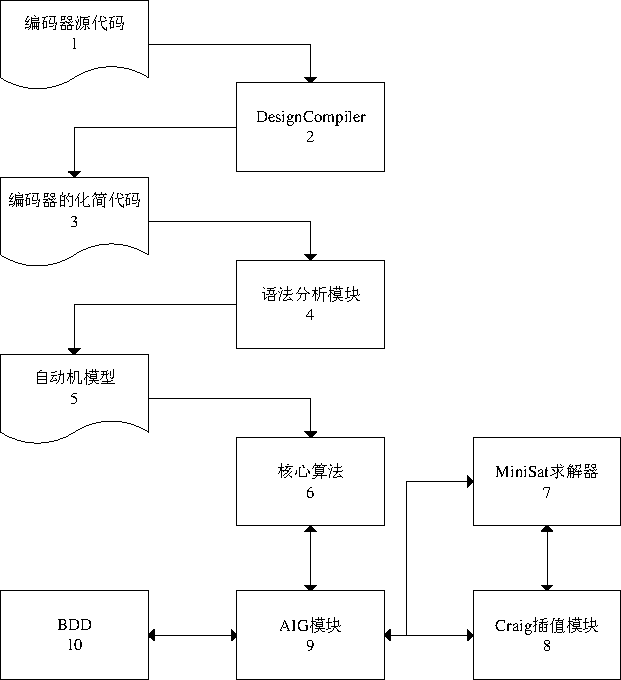
\includegraphics[width=0.8\textwidth]{sysarch}
\caption{原型系统的结构}
\label{fig_sysarch}
\end{figure}

原型系统的结构如图\ref{fig_sysarch}所示。
其中核心算法可以是前述的三个算法,包括:
\begin{enumerate}
\item 第\ref{chap:4}章的面向流控机制的对偶综合算法。
\item 第\ref{chap:5}章的面向流水线的对偶综合算法。
\item 第\ref{chap:6}章的面向流控和流水线的对偶综合算法。
\end{enumerate}


上述三个算法虽然内部结构各不相同,
但是他们与其他各个子系统的关系是完全一样的,
都如图\ref{fig_sysarch}所示。

以下各个小节中我们将详细描述各个子系统的功能。

\subsection{使用DesignCompiler产生编码器的化简代码}

设计编码器的工程师在编写代码的时候,
为了追求更强的表达能力,
更紧凑的代码,
或者更好的可读性等原因,
会使用Verilog语言\upcite{Verilog}提供的各种复杂语法结构。
而开发一个能分析完整的Verilog语法结构的语法分析器会导致大量不必要的额外工作。

因此,
我们选择使用DesignCompiler工具\upcite{DesignCompiler}中自带的完整语法分析器来分析复杂的源代码。

然后我们在DesignCompiler中,
将语法分析的结果映射到DesignCompiler自带的LSI10K单元库中。
为了在保持语义的前提下进一步简化分析结果的语法形式,
我们限制在该映射过程中只能使用与门和非门两种组合逻辑单元。

然后我们将映射的结果导出为一个相对较大,
但是结构非常简单的Verilog源代码文件。
其中只包含一种与门,一种非门和一种寄存器。
这就极大的简化了后继的语法分析程序的设计。


\subsection{语法分析模块}
我们使用OCaml语言自带的词法分析工具OCamllex和语法分析工具OCamlyacc,
创建了针对上述简化的编码器代码的词法和语法分析程序。
词法分析程序的代码在\url{https://github.com/shengyushen/compsyn/blob/master/vp/share/very.mll}。
而语法分析程序的代码在\url{https://github.com/shengyushen/compsyn/blob/master/vp/share/parser.mly}。

分析的结果将被转换为一个有向图$(V,E)$。
其中$V$是节点集合,包含以下类型的节点:
\begin{enumerate}
\item 输入变量$i\in\vec{i}$,
包含1个输出;
\item 输出变量$o\in\vec{o}$,
包含一个输入;
\item 与门,
包含两个输入(A,B)和一个输出Z;
\item 非门,
包含一个输入A和一个输出Z;
\item 寄存器,
包含一个输入D和一个输出Q;
\end{enumerate}

而每条边$e\in E$是单向的,
从一个节点的输出指向另一个节点的输入。
如图\ref{fig_dag}所示。


\begin{figure}[t]
\centering
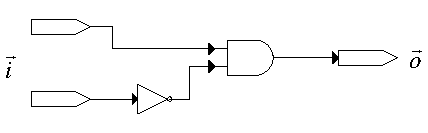
\includegraphics[width=0.8\textwidth]{dag}
\caption{自动机模型的简化描述的例子}
\label{fig_dag}
\end{figure}


\subsection{AIG模块}

AIG是And-Inverter graph的缩写,
即如图\ref{fig_dag}所示的电路结构。
该模块用于构造和维护AIG数据结构,
并负责从AIG到CNF公式的转换。

\subsection{MiniSat求解器}

MiniSat求解器\upcite{EXTSAT}是目前应用最为广泛的SAT求解器。
目前尽管已经有不少新的求解器在性能上超过了MiniSat,
但是由于MiniSat在结构的模块化和可修改性方面具有显著优势,
因此被大量用作理论相关求解器的基础,如数组、未解释函数和线性等式/不等式等。

基于同样的原因,
MiniSat提供了从其自身的C语言内核到OCaml语言的接口。
这为我们在对偶综合算法中调用MiniSat求解器,
并获取其求解结果提供了很大的便利。

\subsection{BDD}
我们选择了学术界广泛使用,
并经过长期验证的CUDD软件包\url{cudd}来处理BDD数据结构。
主要应用于小节\ref{sec_bdd_simp}中描述的基于BDD的化简算法。


\subsection{Craig插值模块}
该模块使用MiniSat求解器的Ocaml接口,
以得到不可满足公式的不可满足证明。
并依据小节\ref{sec_craigimp}中定义\ref{def_gencraig}描述的过程产生Craig插值。

\section{主要流程}
我们在图\ref{fig_sysarch}中的每个方框中都标注了数字,
在以下小节的各个主要流程中,
我们将使用这些数字来指出流程中各个步骤及其顺序。

\subsection{语法分析和有限状态机的构造}
该流程以原始的编码器源代码为输入,
经过$1\to 2\to 3\to 4\to 5$,
最后将产生的有限状态机模型送入核心算法模块。

\subsection{SAT求解}
该步骤从核心算法模块开始,
调用AIG模块产生CNF公式,
送入MiniSat求解器,
并返回结果至核心算法。
经过步骤为$6\to 9\to 7\to 9\to 6$。

\subsection{Craig插值}
该步骤从核心算法模块开始,
调用AIG模块产生CNF公式,
送至Craig插值模块产生相应的不可满足公式。
然后送到MiniSat求解器求解并返回不可满足证明。
然后在Craig插值模块中产生插值结果,
最后返回核心算法。
经过步骤为$6\to 9 \to 8 \to 7 \to 8 \to 9 \to 6$。


\subsection{基于余因子和Craig插值的迭代}
此步骤相当于重复的执行上述的Craig插值操作。
即重复的经过$6\to 9 \to 8 \to 7 \to 8 \to 9 \to 6$。

在完成上述流程之后,
还需要额外调用BDD模块进行结果的化简。

\section{结论}\label{hahahahah}
本章详细描述了系统实现的整体结构,
每个子系统的功能,
以及相互之间的关系。
